% !TeX root = ../../ZF_bmicha_Ana.tex
\subsection{Konvergenzradius}
    \vspace{0.5em}
    \mathbox{
        r = \lim_{n\to\infty} \left\lvert \frac{a_n}{a_{n+1}} \right\rvert
    }
    \begin{center}
            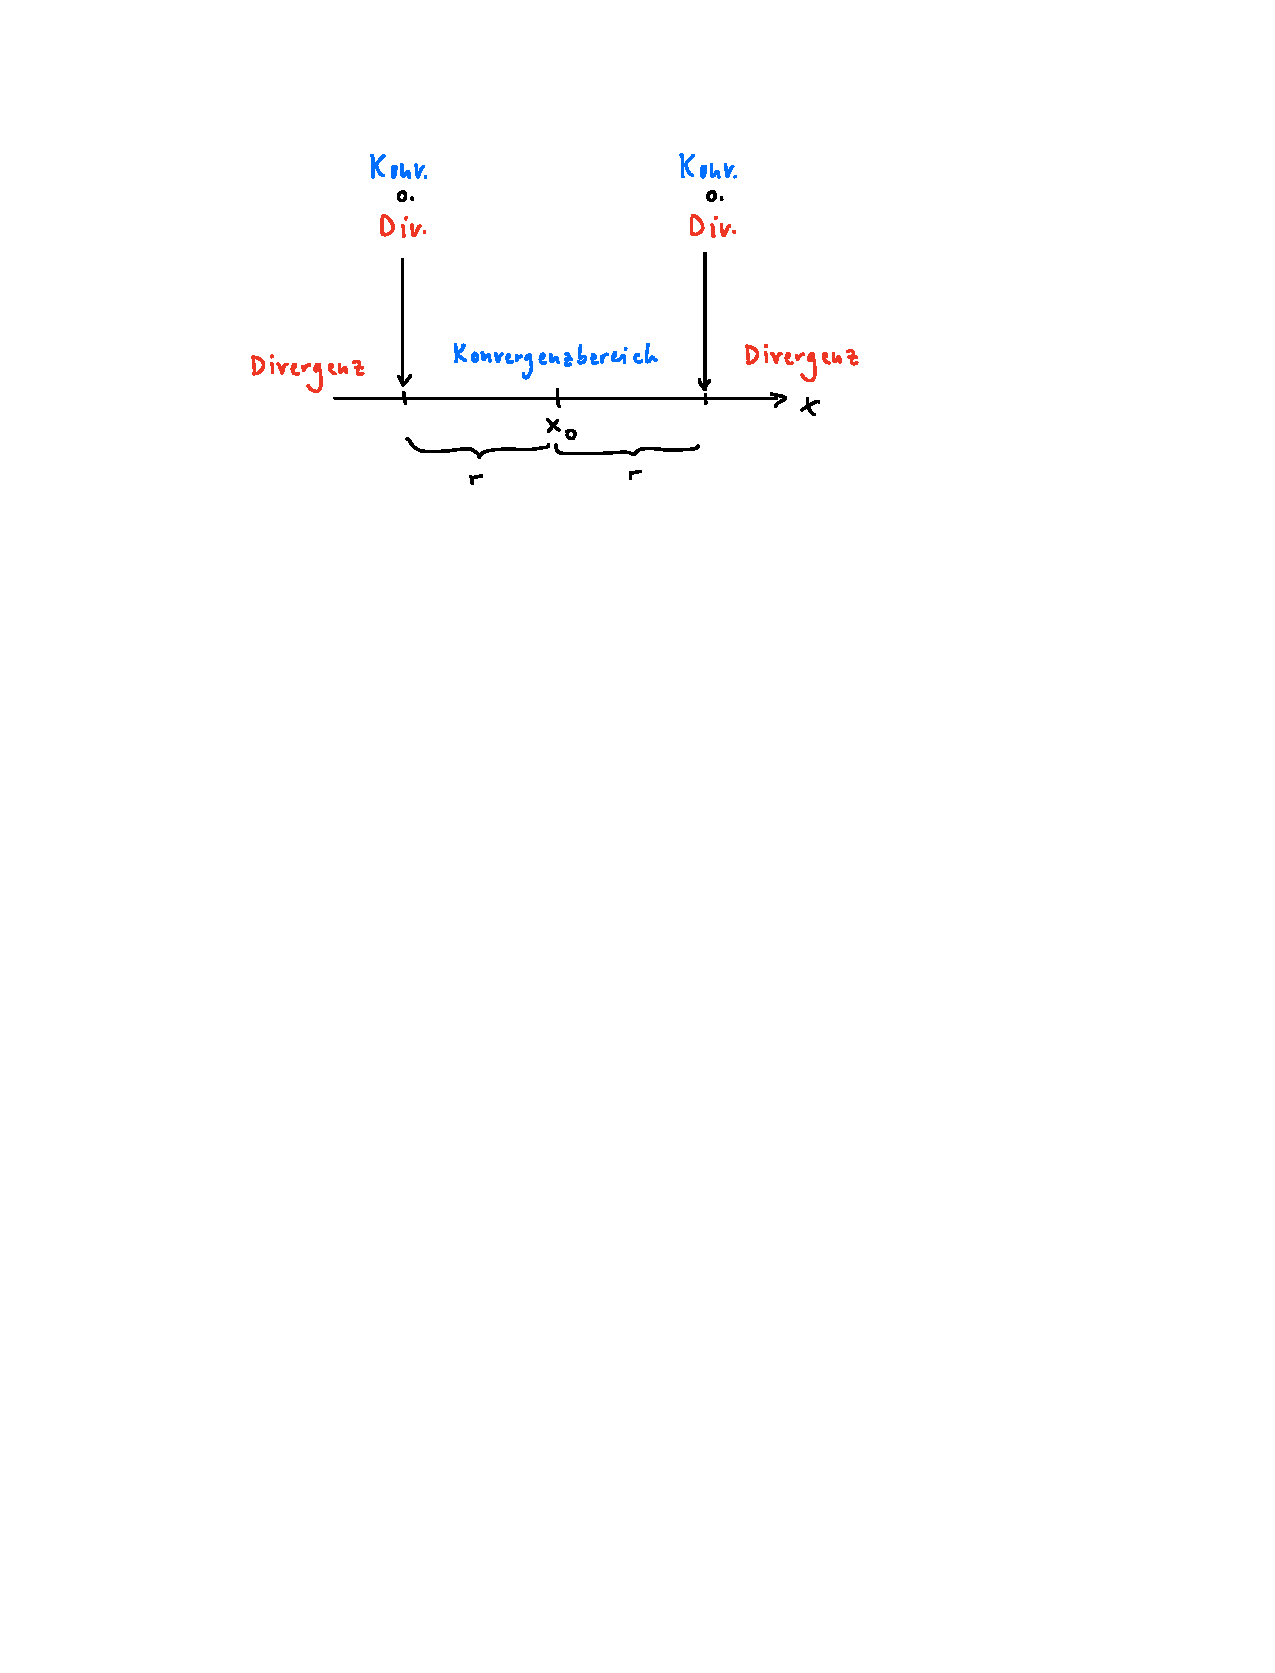
\includegraphics[width=0.65\linewidth]{src/Potenzreihen/konvergenzradius.pdf}
    \end{center}
    Innerhalb vom Konvergenzbereich darf man Potenzreihen \textit{gliedweise}:
    \begin{itemize}
        \item addieren \& subtrahieren
        \item integrieren \& differenzieren
    \end{itemize}